\chapter[Partial Results]{Partial Results}

\section[Results]{Results}

The project has been successful so far, with the website being developed while the scripts were created and tested. This already creates a graphical installer, that will run in most linux distributions, for all the cataloged games developed with SDL 1.

\subsection[Building Scripts]{Building Scripts}

Several games have been tested against the building scripts. Table \ref{tab:script_games} shows which of them were successful in compiling, creating the installers (both GUI and \textit{.deb}) and running. For some games, even with the correct compilation, they wouldn't run as expected, due to logical errors in their code.

\begin{table}[h!]
\centering
\caption{Scripts results}
\label{tab:script_games}
\begin{tabular}{|l|c|c|c|c|}
\hline
\textbf{Game} & \multicolumn{1}{l|}{\textbf{Compiles?}} & \multicolumn{1}{l|}{\textbf{.deb}} & \multicolumn{1}{l|}{\textbf{QT}} & \multicolumn{1}{l|}{\textbf{Runs?}} \\ \hline
Ankhnowledge & s & s & s & s \\ \hline
Post War & s & s & s & s \\ \hline
Jack the Janitor & s & s & s & s \\ \hline
Emperor vs Aliens & s & s & s & s \\ \hline
Ninja Siege & s & s & s & s \\ \hline
Space monkeys & s & s & s & n* \\ \hline
War of the nets & s & s & s & n \\ \hline
Travelling Will & s & s & s & s \\ \hline
\end{tabular}
\end{table}

The game Space Monkeys compiled correctly, however upon running it, the user couldn't do anything and the screens weren't precisely rendered. War of the nets, even compiling without errors, had a segmentation fault after a few seconds with the game open.

\subsection[Platform]{Platform}

The website as of now allows an administrator to upload a game, with its respective information, like supported platform, related media, and installers.


\begin{figure}[!ht]
\centering
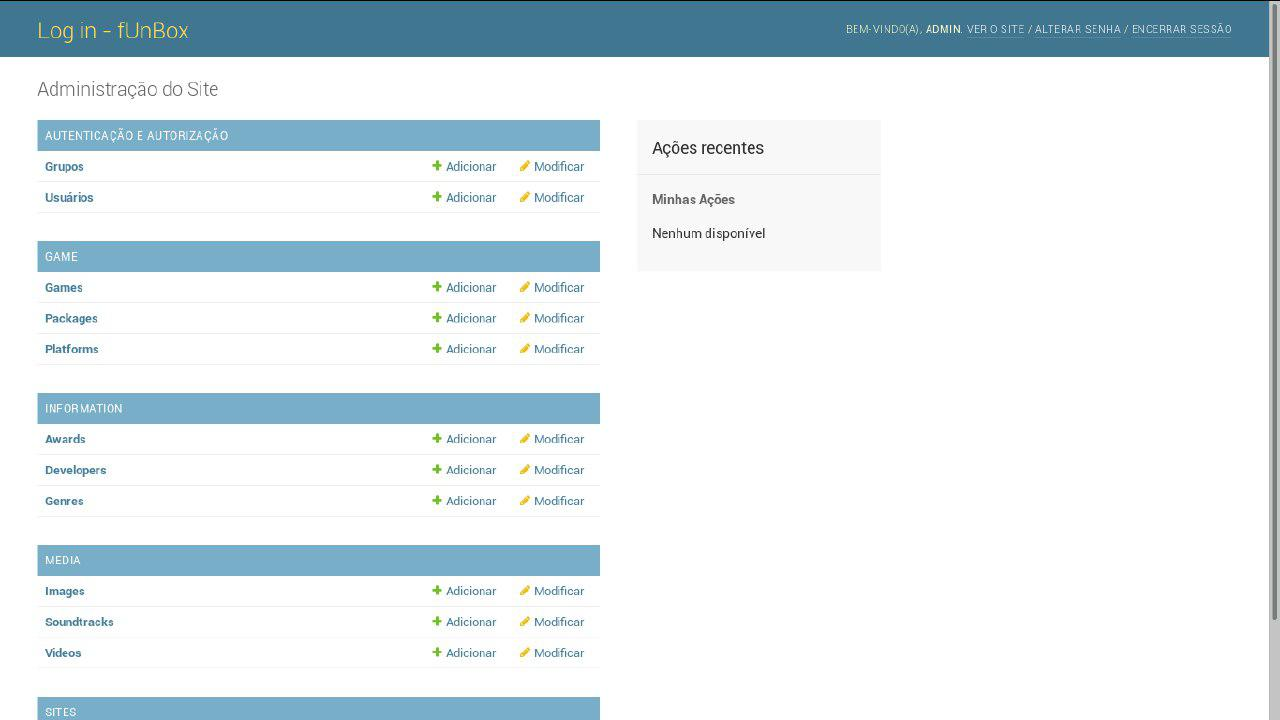
\includegraphics[width=\textwidth,height=\textheight,keepaspectratio]{admin_home_page}
\caption{Administrator home page}
\label{fig:admin_home}
\end{figure}


The general public can see the available games, download them, or comment using a Facebook account.


\section[Future Work]{Future Work}

For the next months it is expected to have the script for the SDL 2 projects finished with support for Windows and MacOS.

Another goal is to have the website running the script automatically when a user links their GitHub repository to the system.


\subsection[Schedule]{Schedule}

The following activities will be developed in the remaining time of the project. They are summarized in the Table \ref{tab:schedule}

\begin{itemize}
\item \textbf{Literature Review} - Review what the literature has on packaging, CMake, game development.
\item \textbf{Add Lua support} - Some of the games have lua as a dependency library that also needs to go in the final package..
\item \textbf{Add other Linux distros support} - Generate at least \textit{.rpm} packages.
\item \textbf{Add MacOS support} - Create install packages for Mac (Apple Systems).
\item \textbf{Add Windows support} - Make a installer (\textit{.exe}) to run on Windows 10 (maybe with some backwards compatibility if possible).
\item \textbf{Integrate to website} - Run the scripts though the website, with GitHub integration.
\item \textbf{Add Darcy's games} - Look for games developed in Darcy Ribeiro campus and test the script on them.
\item \textbf{Code refactoring} - Integrate scripts (SDL 1 and 2), make it more generic and efficient.
\item \textbf{Final adjustments} - Make minor improvements and fixes.
\item \textbf{Write Report} - Report progress and results.
\end{itemize}

\begin{table}[h!]
\centering
\caption{Project Schedule}
\label{tab:schedule}
\begin{tabular}{|l|c|c|c|c|c|c|c|c|c|}
\hline
\textbf{Task} & \multicolumn{1}{l|}{\textbf{Apr}} & \multicolumn{1}{l|}{\textbf{May}} & \multicolumn{1}{l|}{\textbf{Jun}} & \multicolumn{1}{l|}{\textbf{Jul}} & \multicolumn{1}{l|}{\textbf{Ago}} & \multicolumn{1}{l|}{\textbf{Sep}} & \multicolumn{1}{l|}{\textbf{Oct}} & \multicolumn{1}{l|}{\textbf{Nov}} & \multicolumn{1}{l|}{\textbf{Dec}} \\ \hline
Literature Review & x & x & x & x & x &  &  &  &  \\ \hline
Add Lua support &  &  &  & x & x &  &  &  &  \\ \hline
Add other distros support &  &  &  & x & x &  &  &  &  \\ \hline
Add MacOS support &  &  &  &  & x & x &  &  &  \\ \hline
Add Windows support &  &  &  &  & x & x &  &  &  \\ \hline
Integrate to website &  &  &  &  & x & x &  &  &  \\ \hline
Add Darcy's games &  &  &  &  &  & x & x &  &  \\ \hline
Code refactoring &  &  &  &  &  &  & x & x &  \\ \hline
Final adjustments &  &  &  &  &  &  &  & x & x \\ \hline
Write Report &  &  & x &  &  &  &  & x & x \\ \hline
\end{tabular}
\end{table}
